\capitulo{4}{Metodología}

\section{Descripción de los datos}
Para el desarrollo de este proyecto no se han empleado datos ya existentes. Al ejecutar el programa, este nos solicita cuatro datos: nombre completo, año de nacimiento, usuario y contraseña. Una vez estos datos estén completos, el sensor comenzará a realizar lecturas de los valores de presión. Para más información consultar \textit{Anexo D}. En el futuro, cuando se pueda desarrollar la idea de este proyecto se generarán multitud de datos, desde los datos personales del paciente (nombre, apellidos, fecha de nacimiento, número de historia clínica etc) que deberán estar correctamente protegidos con las leyes vigentes del momento (contemplar \textit{Anexo A}), como todos los datos relativos a la presión intracraneal del paciente, que estará continuamente monitorizado. Todos estos datos estarán almacenados en historiales para poder analizarlos, realizar estadísticas y establecer patrones con el objetivo de mejorar la evolución del paciente.
 
\section{Técnicas y herramientas}

El objetivo de esta sección es hacer una breve recopilación tanto de las técnicas y aplicaciones empleadas para desarrollar este proyecto como de las herramientas necesarias para ello.

\subsection{Aplicaciones}

A continuación se presentan las aplicaciones gratuitas empleadas para desarrollar este trabajo acompañadas de una breve descripción de cada una de ellas. Algunas como Overleaf, GitHub o Arduino, han sido utilizadas a lo largo del grado.

\begin{itemize}
    \item \textbf{Overleaf} \cite{overleaf}: es una plataforma colaborativa en línea que utiliza LaTex para la publicación y redacción de documentos. LaTex es una herramienta para componer textos de aspecto profesional convirtiendo un documento de texto sin formato formado por comandos LaTex y texto en un archivo PDF. Para llevar a cabo esta conversión, LaTex emplea un software denominado motor TeX por lo tanto el usuario solo debe centrarse en el contenido del documento sin preocuparse de la apariencia visual. En este proyecto se ha empleado para desarrollar este documento y los anexos.
    
    \item \textbf{GitHub} \cite{github}: es una plataforma en línea gratuita de desarrollo de software colaborativo que utiliza el sistema de control de versiones Git cuya función es realizar un seguimiento de los cambios que se producen en los archivos. Es de código abierto y permite a los usuarios trabajar juntos en proyectos de software, facilitando el seguimiento de posibles cambios en el código, colaboración en equipo y organización de proyectos. Para este proyecto se ha creado un repositorio público en el que a través de tareas (issues) se ha ido organizando el desarrollo del mismo.
    
    \item \textbf{Arduino} \cite{arduino}: es una plataforma de código abierto basada en hardware y software libre. Es flexible, fácil de usar y de bajo coste, por lo que habitualmente es elegida para llevar a cabo distintos proyectos electrónicos. Arduino cuenta con un entorno de programación, Arduino IDE, con el que el usuario puede crear diferentes aplicaciones para las placas dándole todo tipo de utilidades. Esta placa puede ser programada tanto en Windows como en macOS y GNU/Linux y emplea un lenguaje de programación similar a C++ pero simplificado. Arduino ha sido elegido para realizar este proyecto principalmente por su sencillez y bajo coste.
    
    \item \textbf{Biorender} \cite{biorender}: es un programa online gratuito para elaborar imágenes científicas. En este proyecto se ha utilizado para crear alguna imagen como por ejemplo la Figura \ref{fig:tipos_espina}.

    \item \textbf{Unfold} \cite{unfold}: es un aplicación de edición de fotos y vídeos que se ha empleado para elaborar los vídeos contenidos en la carpeta demostraciones del \href{https://github.com/CeliaValladolid/TFG_Valvula_Derivacion_VentriculoPeritoneal}{Repositorio}.
    
\end{itemize}

\subsection{Herramientas}
Al igual que en el apartado anterior, se citarán las herramientas necesarias para llevar a cabo este proyecto así como un breve resumen de todas ellas.

\begin{itemize}
    \item \textbf{Placa de arduino UNO R3} \cite{placa}: es una placa de desarrollo de código abierto que integra un microcontrolador ATmega328P de alta eficiencia \cite{placa}. En la Figura \ref{fig:placa_Arduino} podemos observar la placa empleada para el proyecto junto con la indicación de cada uno de sus componentes.
    \begin{figure}[h]
    \centering
    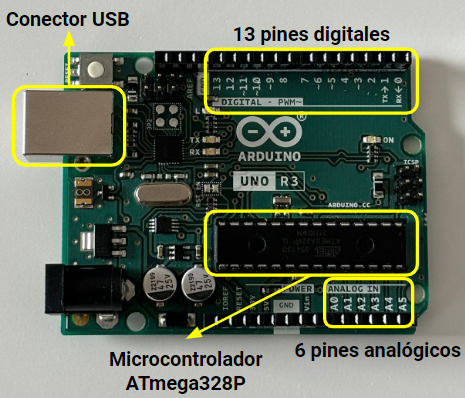
\includegraphics[width=0.6\textwidth]{img/PLACAPARTES.PNG}
    \caption{Placa de Arduino UNO R3. Imagen Propia}
    \label{fig:placa_Arduino}
\end{figure}

    \item \textbf{Cables}: cables empleados para realizar el cableado del proyecto, de la placa de Arduino a la protoboard o a los componentes que sea necesario. Hemos empleado cables macho-hembra\footnote{Los cables macho-hembra son cables que presentan un pincho en un lado y un hueco en el otro \cite{cables}} para llevar a cabo algunas conexiones. Podemos observarlos en la Figura \ref{fig:cables}.
    \begin{figure}[h]
    \centering
    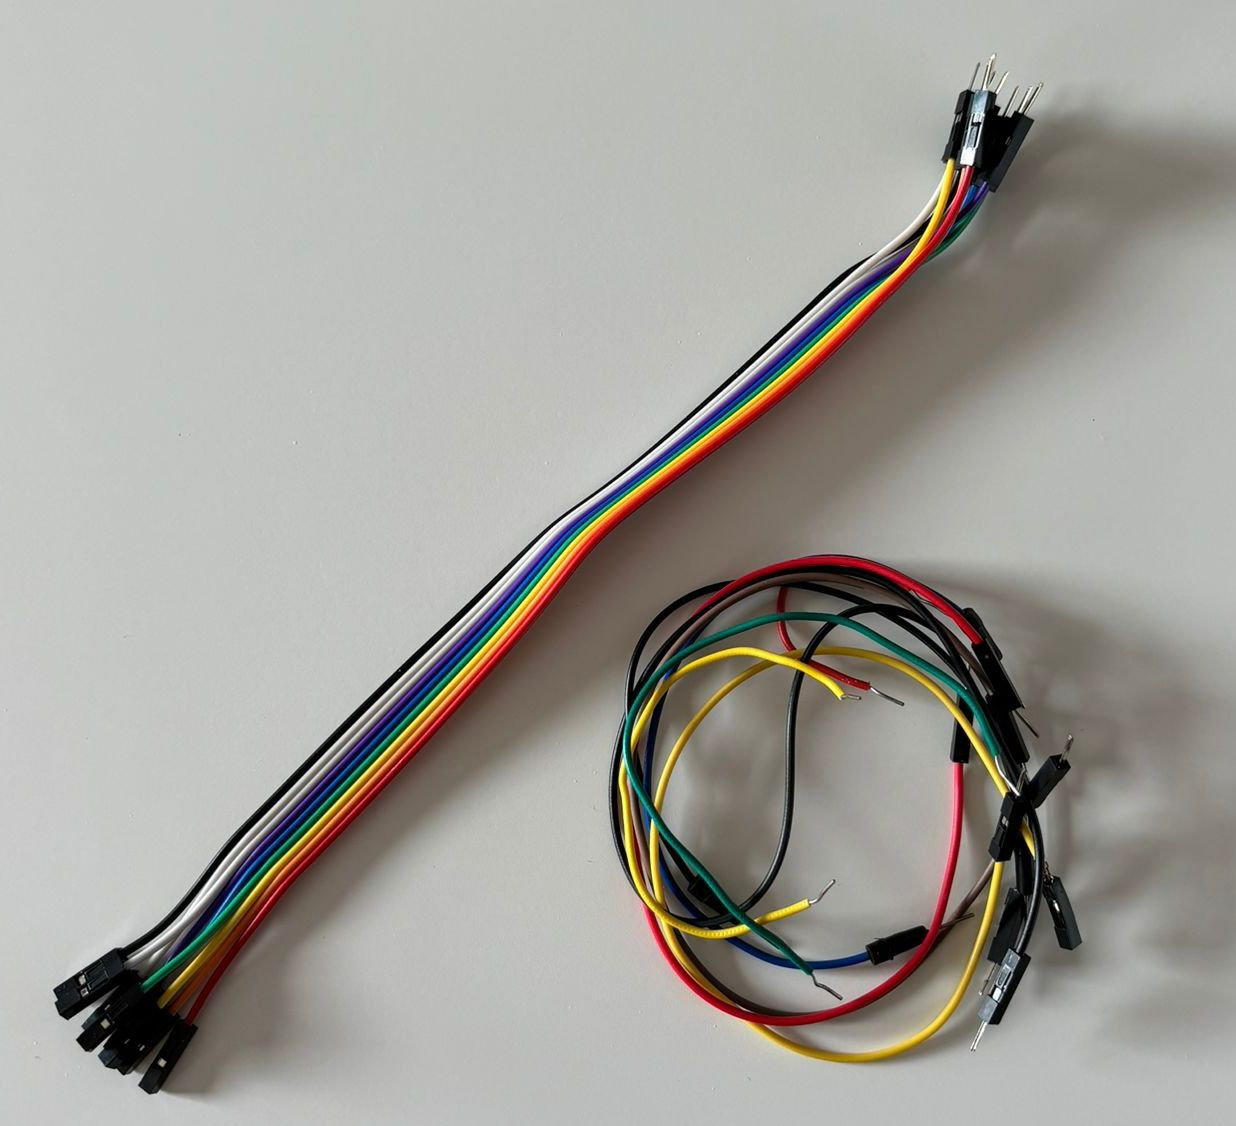
\includegraphics[width=0.6\textwidth]{img/cables.jpg}
    \caption{Cables. Imagen Propia}
    \label{fig:cables}
\end{figure}

    \item \textbf{ProtoBoard}: también conocida como placa de pruebas, se trata de una placa electrónica cuya función es el prototipado de circuitos y conexiones. Una protoboard consta de un número variable de clavijas (según el tamaño escogido) en las cuáles se insertan los diferentes componentes electrónicos y de 4 filas , dos superiores y dos inferiores, marcadas con el signo + y - encargadas de llevar la corriente y la toma tierra al circuito. Todos los pines de las diferentes filas están conectados entre sí. En la Figura \ref{fig:protoboard} podemos observar el aspecto de este componente.
    \begin{figure}[h]
    \centering
    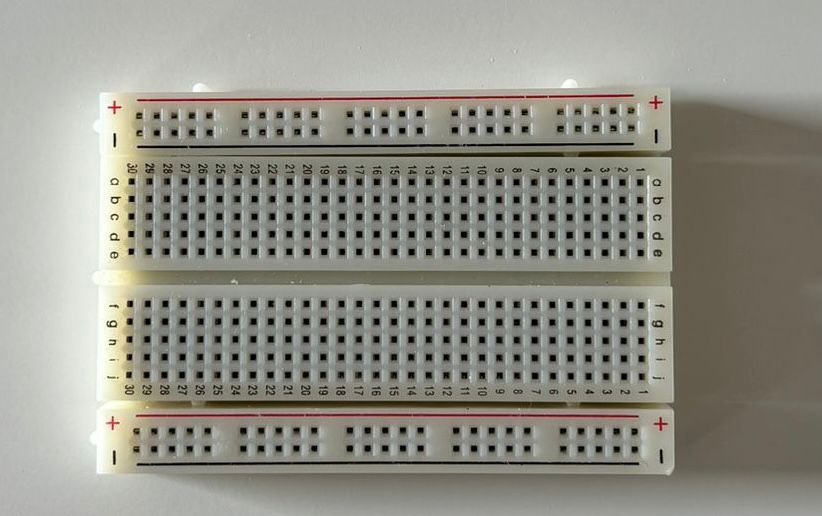
\includegraphics[width=0.6\textwidth]{img/proto.jpg}
    \caption{ProtoBoard, placa de pruebas. Imagen Propia}
    \label{fig:protoboard}
\end{figure}

    \item \textbf{Cable USB}: cable que permite conectar la placa de Arduino con un ordenador y así ejecutar las instrucciones programadas. Lo podemos observar en la Figura \ref{fig:USB}.
    \begin{figure}[h]
    \centering
    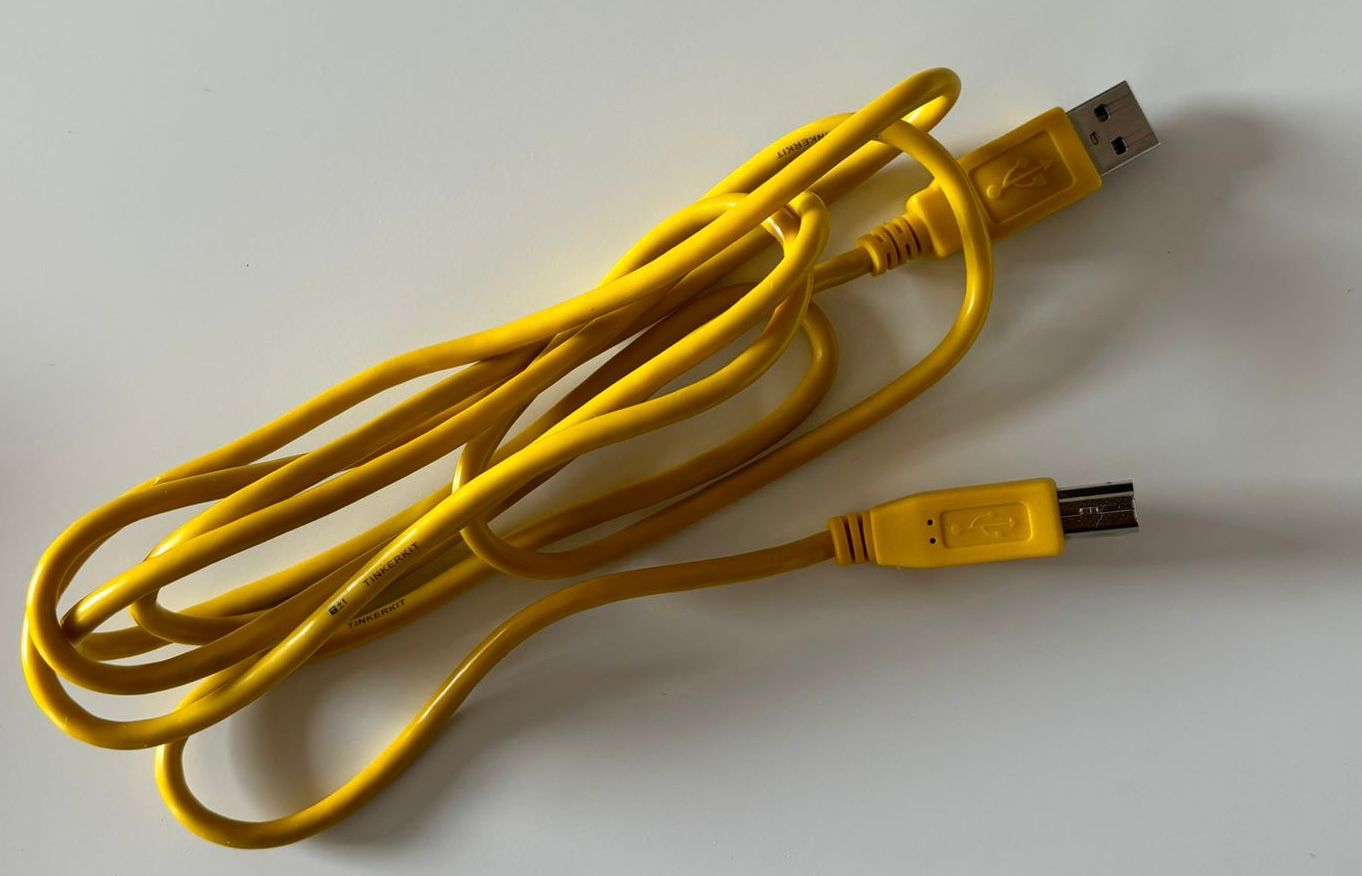
\includegraphics[width=0.6\textwidth]{img/usb.jpg}
    \caption{Cable USB. Imagen Propia}
    \label{fig:USB}
\end{figure}

    \item \textbf{Sensor de presión NPX MPX5010DP}: se trata de un sensor de presión diferencial de silicio integrado de doble puerto en un encapsulado SIP de 6 pines \cite{npx}. Según la Figura \ref{fig:sensor_pres} el pin 1 es el de la izquierda, el que presenta una muesca y el que se conecta a un pin analógico de nuestro Arduino. Los pines 2 y 3 son los que están a continuación y se conectan a GND y 5V respectivamente. Este sensor entrega en su salida un voltaje de 0-5 V, lo que le hace ideal para microcontroladores \cite{npx_}. 
    \begin{figure}[h]
    \centering
    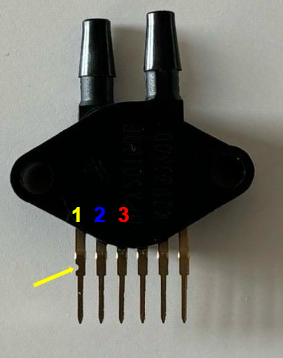
\includegraphics[width=0.35\textwidth]{img/sensor_1.PNG}
    \caption{Sensor de presión NPX MPX5010DP. Imagen Propia}
    \label{fig:sensor_pres}
    \end{figure}
    En la Tabla \ref{tab:caracteristicas_sensor} podemos ver recogidas las principales características del sensor:
    
    \begin{table}[htbp]
    \centering
    \begin{tabular}{>{\raggedright\arraybackslash}p{0.9\linewidth}}
    \hline
    \rowcolor{blue!20}
    \multicolumn{1}{c}{\textbf{Características del sensor NPX MPX5010DP}} \\
    \hline
    Calibración, compensación de temperatura y acondicionamiento de señal en chip \\
    Configuración diferencial \\
    Error máximo de 5,0\% entre 0°C y 85°C \\
    Diseño de una pieza de epoxi duradera \\
    Compensación de temperatura de -40°C a 125°C \\
    Galga extensiométrica de esfuerzo cortante de silicio patentada \\
    Rango de presión de 0KPa a 10KPa \\
    Rango de tensión de alimentación de 4,75VDC a 5,25VDC \\
    Sensibilidad de 450mV/mm \\
    Tiempo de respuesta de 1ms \\
    \hline
    \end{tabular}
    \caption{Características del sensor NPX MPX5010DP \cite{npx}}
    \label{tab:caracteristicas_sensor}
    \end{table}
    

    \item \textbf{Mini bomba}: mini bomba de agua sumergible que presenta un voltaje DC 3-5V y una corriente de 100-200 mA. Viene acompañada de una manguera de plástico para que circule el agua de un recipiente a otro. Ambos elementos los podemos observar en la Figura \ref{fig:mini_bomba}.
    \begin{figure}[h]
    \centering
    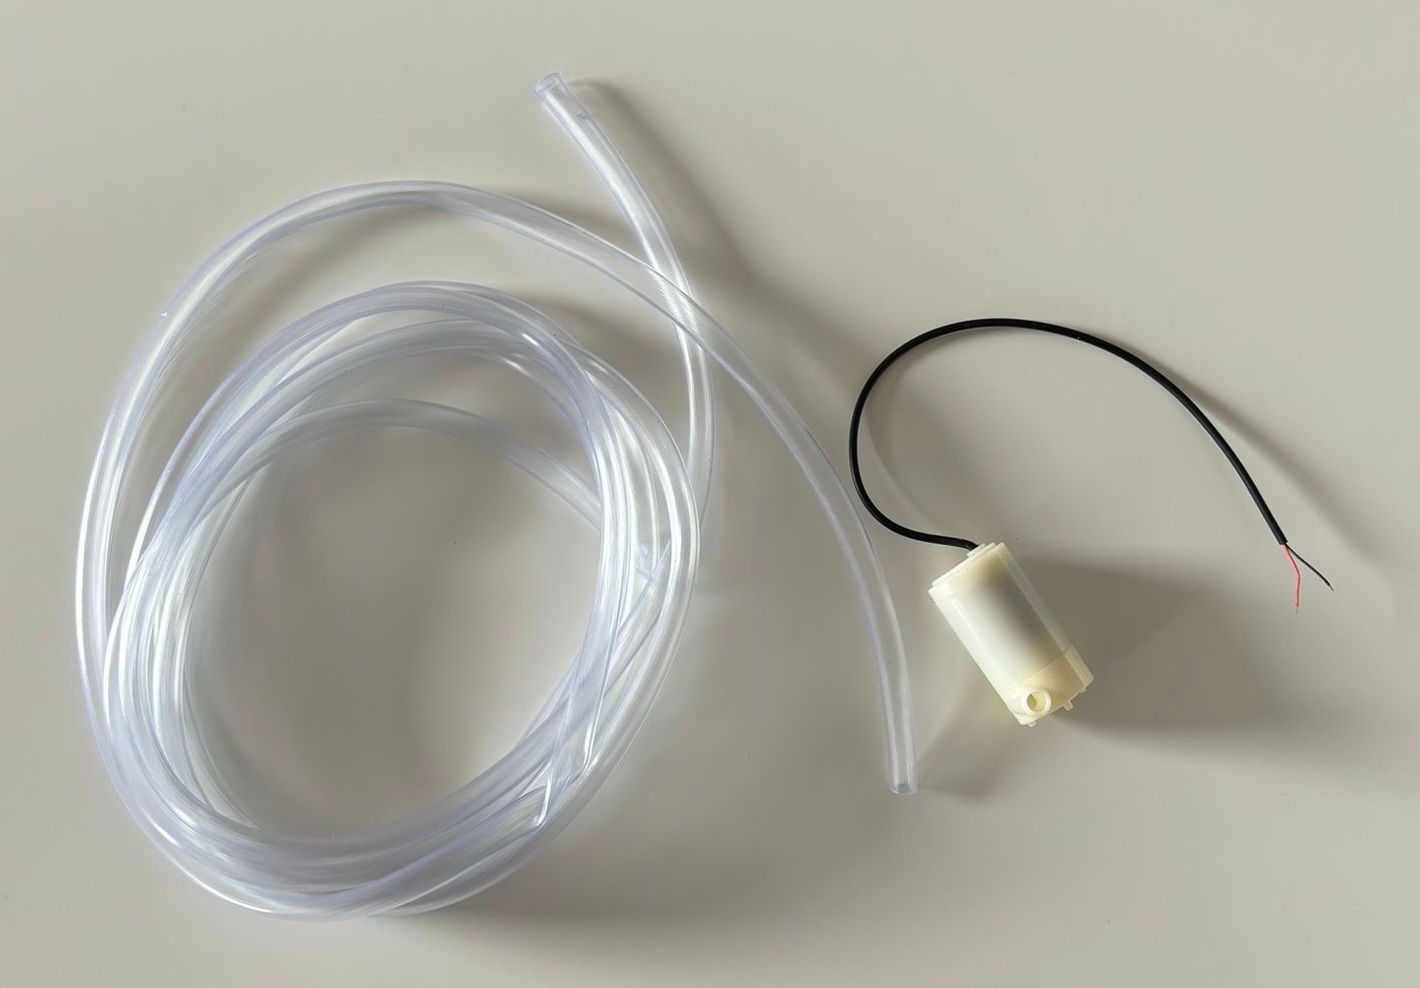
\includegraphics[width=0.65\textwidth]{img/bomba.jpg}
    \caption{Mini bomba. Imagen Propia}
    \label{fig:mini_bomba}
\end{figure}

    \item \textbf{Relé}: es un componente electromagnético que actúa como un interruptor, permitiendo el paso de la corriente cuando se encuentra cerrado e interrumpiendo este flujo cuando permanece abierto. Este dispositivo no se acciona de forma manual sino a través de una señal eléctrica. En su interior cuenta con una bobina conectada a la corriente y cuando ésta se acciona genera un campo electromagnético que provoca el cierre del contacto del relé, permitiendo así que circule la corriente. Cuando dejamos de suministrar corriente a la bobina, el contacto se abre,desaparece el campo electromagnético y el dispositivo que estamos controlando queda privado de corriente para seguir en funcionamiento \cite{rele}. En este proyecto emplearemos un relé de un canal para activar y desactivar la mini bomba. En la Figura \ref{fig:rele} podemos observar los pines y contactos con los que cuenta.
    \begin{figure}[h]
    \centering
    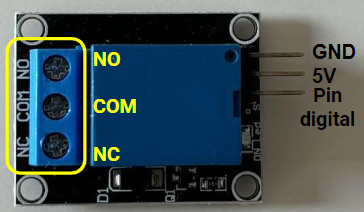
\includegraphics[width=0.6\textwidth]{img/relepartes.PNG}
    \caption{Relé. Imagen Propia}
    \label{fig:rele}
\end{figure}

    \item \textbf{Portapilas}: compartimento para albergar tres pilas en serie de 1,5V cada una consiguiendo así un voltaje total de 4,5V para poder alimentar nuestro circuito. Es apto para pilas LR6 AA (FR6, HR6, LR6) e incluye un interruptor ON/OFF. Lo podemos observar en la Figura \ref{fig:portapilas}.
    \begin{figure}[h]
    \centering
    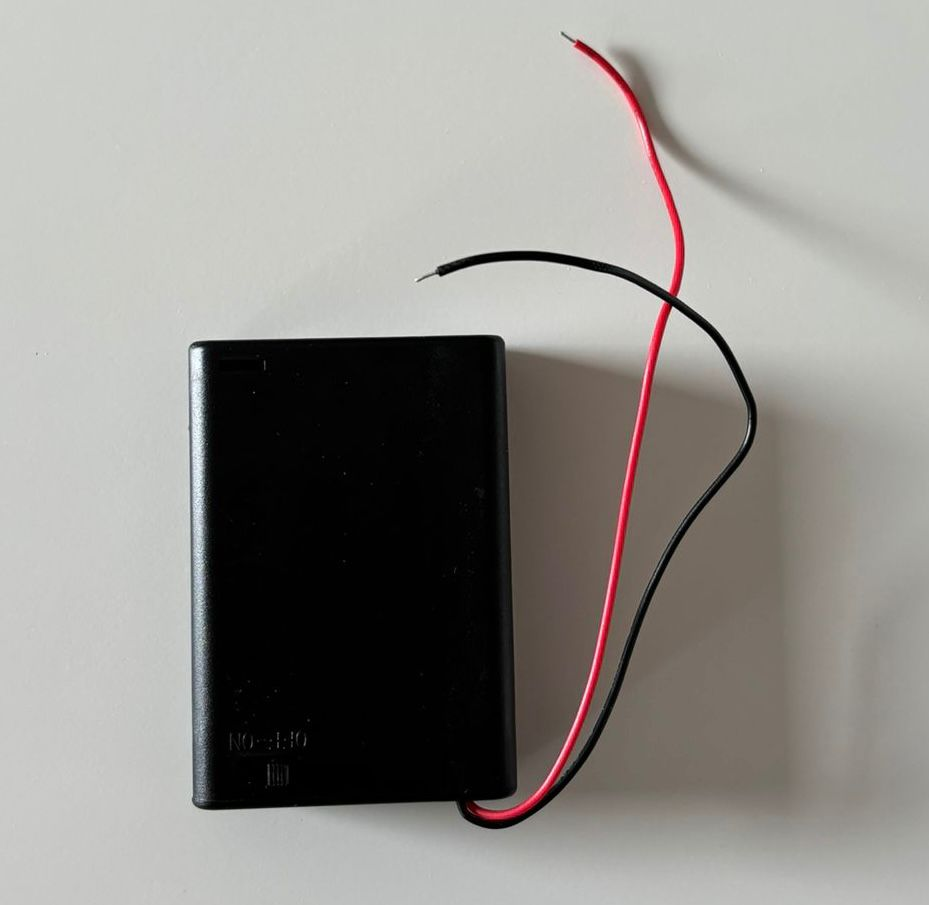
\includegraphics[width=0.6\textwidth]{img/portapilas.jpg}
    \caption{Portapilas. Imagen Propia}
    \label{fig:portapilas}
\end{figure}

    \item \textbf{Pilas}: pilas LR6 AA empleadas para alimentar nuestro circuito. Las podemos observar en la Figura \ref{fig: pilas}.
    \begin{figure}[h]
    \centering
    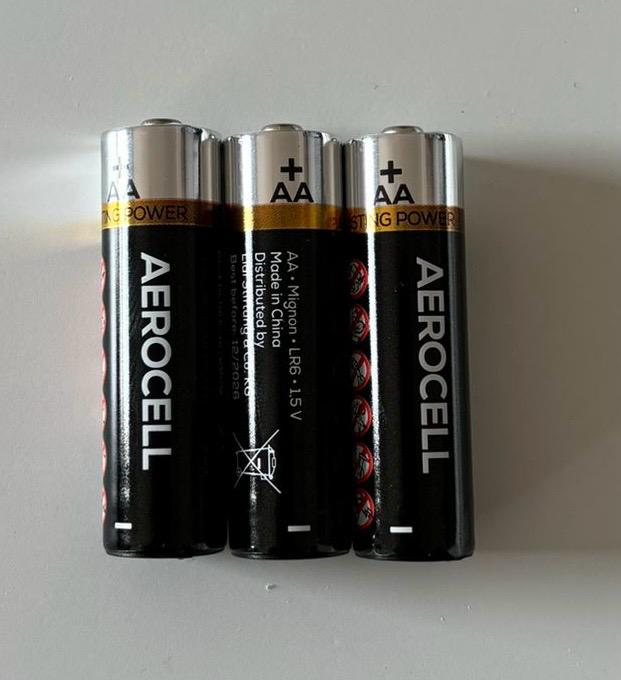
\includegraphics[width=0.5\textwidth]{img/pilas.jpg}
    \caption{Pilas. Imagen Propia}
    \label{fig: pilas}
\end{figure}

\end{itemize}
